\section{GtkExpression}\label{gtkexpression}

GtkExpression is a fundamental type. It is not a descendant of GObject.
GtkExpression provides a way to describe references to values.
GtkExpression needs to be evaluated to obtain a value.

It is similar to arithmetic calculation.

\begin{lstlisting}
1 + 2 = 3
\end{lstlisting}

\passthrough{\lstinline!1+2!} is an expression. It shows the way how to
calculate. \passthrough{\lstinline!3!} is the value comes from the
expression. Evaluation is to calculate the expression and get the value.

GtkExpression is a way to get a value. Evaluation is like a calculation.
A value is got by evaluating the expression.

\subsection{Constant expression}\label{constant-expression}

A constant expression (GtkConstantExpression) provides constant value or
instance when it is evaluated.

\begin{lstlisting}[language=C]
  GValue value = G_VALUE_INIT;
  expression = gtk_constant_expression_new (G_TYPE_INT,100);
  gtk_expression_evaluate (expression, NULL, &value);
\end{lstlisting}

\begin{itemize}
\tightlist
\item
  GtkExpression uses GValue to hold a value. GValue is a structure and
  container to hold a type and value. It must be initialized with
  \passthrough{\lstinline!G\_VALUE\_INIT!}, first. Be careful that
  \passthrough{\lstinline!value!} is a structure, not a pointer to a
  structure.
\item
  Constant expression is created with
  \passthrough{\lstinline!gtk\_constant\_expression\_new!} function. The
  parameter of the function is a type (GType) and a value (or instance).
  This expression holds a constant value.
  \passthrough{\lstinline!G\_TYPE\_INT!} is a type that is registered to
  the type system. It is integer type. Some types are shown in the
  following table.
\item
  \passthrough{\lstinline!gtk\_expression\_evaluate!} evaluates the
  expression. It has three parameters, the expression to evaluate,
  \passthrough{\lstinline!this!} instance and a pointer to a GValue for
  being set with the value. \passthrough{\lstinline!this!} instance
  isn't necessary for constant expressions. Therefore, the second
  argument is NULL. \passthrough{\lstinline!gtk\_expression\_evaluate!}
  returns TRUE if it successfully evaluates the expression. Otherwise it
  returns FALSE.
\item
  If it returns TRUE, the GValue \passthrough{\lstinline!value!} is set
  with the value of the expression. The type of the value is int.
\end{itemize}

\begin{longtable}[]{@{}llll@{}}
\toprule\noalign{}
GType & C type & type name & notes \\
\midrule\noalign{}
\endhead
\bottomrule\noalign{}
\endlastfoot
G\_TYPE\_CHAR & char & gchar & \\
G\_TYPE\_BOOLEAN & int & gboolean & \\
G\_TYPE\_INT & int & gint & \\
G\_TYPE\_FLOAT & float & gfloat & \\
G\_TYPE\_DOUBLE & double & gdouble & \\
G\_TYPE\_POINTER & void * & gpointer & general pointer \\
G\_TYPE\_STRING & char * & gchararray & null-terminated Cstring \\
G\_TYPE\_OBJECT & & GObject & \\
GTK\_TYPE\_WINDOW & & GtkWindow & \\
\end{longtable}

A sample program \passthrough{\lstinline!exp\_constant\_simple.c!} is in
\passthrough{\lstinline!src/expression!} directory.

\begin{lstlisting}[language=C, numbers=left]
#include <gtk/gtk.h>

int
main (int argc, char **argv) {
  GtkExpression *expression;
  GValue value = G_VALUE_INIT;

  /* Create an expression */
  expression = gtk_constant_expression_new (G_TYPE_INT,100);
  /* Evaluate the expression */
  if (gtk_expression_evaluate (expression, NULL, &value))
    g_print ("The value is %d.\n", g_value_get_int (&value));
  else
    g_print ("The constant expression wasn't evaluated correctly.\n");
  gtk_expression_unref (expression);
  g_value_unset (&value);

  return 0;
}
\end{lstlisting}

\begin{itemize}
\tightlist
\item
  9: A constant expression is created. It holds an int value 100. The
  variable \passthrough{\lstinline!expression!} points the expression.
\item
  11-14: Evaluates the expression. If it successes, show the value to
  the stdout. Otherwise show an error message.
\item
  15-16: Releases the expression and unsets the GValue.
\end{itemize}

Constant expression is usually used to give a constant value or instance
to another expression.

\subsection{Property expression}\label{property-expression}

A property expression (GtkPropertyExpression) looks up a property in a
GObject instance. For example, a property expression that refers
``label'' property in a GtkLabel object is created like this.

\begin{lstlisting}[language=C]
expression = gtk_property_expression_new (GTK_TYPE_LABEL, another_expression, "label");
\end{lstlisting}

The second parameter \passthrough{\lstinline!another\_expression!} is
one of:

\begin{itemize}
\tightlist
\item
  An expression that gives a GtkLabel instance when it is evaluated.
\item
  NULL. When NULL is given, a GtkLabel instance will be given when it is
  evaluated. The instance is called \passthrough{\lstinline!this!}
  object.
\end{itemize}

For example,

\begin{lstlisting}[language=C]
label = gtk_label_new ("Hello");
another_expression = gtk_constant_expression_new (GTK_TYPE_LABEL, label);
expression = gtk_property_expression_new (GTK_TYPE_LABEL, another_expression, "label");
\end{lstlisting}

If \passthrough{\lstinline!expression!} is evaluated, the second
parameter \passthrough{\lstinline!another\_expression!} is evaluated in
advance. The value of \passthrough{\lstinline!another\_expression!} is
the \passthrough{\lstinline!label!} (GtkLabel instance). Then,
\passthrough{\lstinline!expression!} looks up ``label'' property of the
label and the evaluation results in ``Hello''.

In the example above, the second argument of
\passthrough{\lstinline!gtk\_property\_expression\_new!} is another
expression. But the second argument can be NULL. If it is NULL,
\passthrough{\lstinline!this!} instance is used instead.
\passthrough{\lstinline!this!} is given by
\passthrough{\lstinline!gtk\_expression\_evaluate!} function.

There's a simple program
\passthrough{\lstinline!exp\_property\_simple.c!} in
\passthrough{\lstinline!src/expression!} directory.

\begin{lstlisting}[language=C, numbers=left]
#include <gtk/gtk.h>

int
main (int argc, char **argv) {
  GtkWidget *label;
  GtkExpression *expression;
  GValue value = G_VALUE_INIT;

  gtk_init ();
  label = gtk_label_new ("Hello world.");
  /* Create an expression */
  expression = gtk_property_expression_new (GTK_TYPE_LABEL, NULL, "label");
  /* Evaluate the expression */
  if (gtk_expression_evaluate (expression, label, &value))
    g_print ("The value is %s.\n", g_value_get_string (&value));
  else
    g_print ("The property expression wasn't evaluated correctly.\n");
  gtk_expression_unref (expression);
  g_value_unset (&value);

  return 0;
}
\end{lstlisting}

\begin{itemize}
\tightlist
\item
  9-10: \passthrough{\lstinline!gtk\_init!} initializes GTK GUI toolkit.
  It isn't usually necessary because the GtkApplication default startup
  handler does the initialization. A GtkLabel instance is created with
  the text ``Hello world.''.
\item
  12: A property expression is created. It looks a ``label'' property of
  a GtkLabel instance. But at the creation, no instance is given because
  the second argument is NULL. The expression just knows how to take the
  property from a future-given GtkLabel instance.
\item
  14-17: The function
  \passthrough{\lstinline!gtk\_expression\_evaluate!} evaluates the
  expression with a `this' instance \passthrough{\lstinline!label!}. The
  result is stored in the GValue \passthrough{\lstinline!value!}. The
  function \passthrough{\lstinline!g\_value\_get\_string!} gets a string
  from the GValue. But the string is owned by the GValue so you must not
  free the string.
\item
  18-19: Releases the expression and unset the GValue. At the same time
  the string in the GValue is freed.
\end{itemize}

If the second argument of
\passthrough{\lstinline!gtk\_property\_expression\_new!} isn't NULL, it
is another expression. The expression is owned by a newly created
property expression. So, when the expressions are useless, you just
release the last expression. Then it releases another expression it has.

\subsection{Closure expression}\label{closure-expression}

A closure expression calls closure when it is evaluated. A closure is a
generic representation of a callback (a pointer to a function). For
information about closure, see
\href{https://docs.gtk.org/gobject/concepts.html\#the-gobject-messaging-system}{GObject
API Reference -- The GObject messaging system}. There are simple closure
example files \passthrough{\lstinline!closure.c!} and
\passthrough{\lstinline!closure\_each.c!} in the
\passthrough{\lstinline!src/expression!} directory.

There are two types of closure expressions, GtkCClosureExpression and
GtkClosureExpression. They corresponds to GCClosure and GClosure
respectively. When you program in C language, GtkCClosureExpression and
GCClosure are appropriate.

A closure expression is created with
\passthrough{\lstinline!gtk\_cclosure\_expression\_new!} function.

\begin{lstlisting}[language=C]
int
callback (GObject *object, int x, const char *s)
\end{lstlisting}

The following is \passthrough{\lstinline!exp\_closure\_simple.c!} in
\passthrough{\lstinline!src/expression!}.

\begin{lstlisting}[language=C, numbers=left]
#include <gtk/gtk.h>

static int
calc (GtkLabel *label) { /* this object */
  const char * s;
  int i, j;

  s = gtk_label_get_text (label); /* s is owned by the label. */
  sscanf (s, "%d+%d", &i, &j);
  return i+j;
}

int
main (int argc, char **argv) {
  GtkExpression *expression;
  GValue value = G_VALUE_INIT;
  GtkLabel *label;

  gtk_init ();
  label = GTK_LABEL (gtk_label_new ("123+456"));
  g_object_ref_sink (label);
  expression = gtk_cclosure_expression_new (G_TYPE_INT, NULL, 0, NULL,
                 G_CALLBACK (calc), NULL, NULL);
  if (gtk_expression_evaluate (expression, label, &value)) /* 'this' object is the label. */
    g_print ("%d\n", g_value_get_int (&value));
  else
    g_print ("The closure expression wasn't evaluated correctly.\n");
  gtk_expression_unref (expression);
  g_value_unset (&value);
  g_object_unref (label);
  
  return 0;
}
\end{lstlisting}

\begin{itemize}
\tightlist
\item
  3-11: A call back function. The parameter is only one and it is a
  `this' object. It is a GtkLabel and its label is assumed to be
  ``(number)+(number)''.
\item
  8-10: Retrieves two integers from the label and returns the sum of
  them. This function has no error report. If you want to return error
  report, change the return value type to be a pointer to a structure of
  gboolean and integer. One for error and the other for the sum. The
  first argument of
  \passthrough{\lstinline!gtk\_cclosure\_expression\_new!} is
  \passthrough{\lstinline!G\_TYPE\_POINTER!}. There is a sample program
  \passthrough{\lstinline!exp\_closure\_with\_error\_report!} in
  \passthrough{\lstinline!src/expression!} directory.
\item
  19: The function `gtk\_init`` initializes GTK. It is necessary for
  GtkLabel.
\item
  20: A GtkLabel instance is created with ``123+456''.
\item
  21: The instance has floating reference. It is changed to an ordinary
  reference count.
\item
  22-23: Creates a closure expression. Its return value type is
  \passthrough{\lstinline!G\_TYPE\_INT!} and no parameters or `this'
  object.
\item
  24: Evaluates the expression with the label as a `this' object.
\item
  25: If the evaluation successes, the sum of ``123+456'', which is 579,
  is shown.
\item
  27: If it fails, an error message appears.
\item
  28-30: Releases the expression and the label. Unsets the value.
\end{itemize}

Closure expression is flexible than other type of expression because you
can specify your own callback function.

\subsection{GtkExpressionWatch}\label{gtkexpressionwatch}

GtkExpressionWatch is a structure, not an object. It represents a
watched GtkExpression. Two functions create GtkExpressionWatch
structure. They are \passthrough{\lstinline!gtk\_expression\_bind!} and
\passthrough{\lstinline!gtk\_expression\_watch!}.

\subsubsection{gtk\_expression\_bind
function}\label{gtk_expression_bind-function}

This function binds the target object's property to the expression. If
the value of the expression changes, the property reflects the value
immediately.

\begin{lstlisting}[language=C]
GtkExpressionWatch*
gtk_expression_bind (
  GtkExpression* self,
  GObject* target,
  const char* property,
  GObject* this_
)
\end{lstlisting}

This function takes the ownership of the expression. So, if you want to
own the expression, call
\passthrough{\lstinline!gtk\_expression\_ref ()!} to increase the
reference count of the expression. And you should unref it when it is
useless. If you don't own the expression, you don't care about releasing
the expression.

An example \passthrough{\lstinline!exp\_bind.c!} and
\passthrough{\lstinline!exp\_bind.ui!} is in
\passthrough{\lstinline!src/expression!} directory.

\begin{figure}
\centering
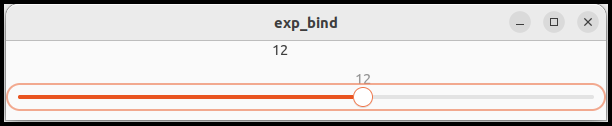
\includegraphics[width=9.2cm,height=1.9cm]{../image/exp_bind.png}
\caption{exp\_bind}
\end{figure}

It includes a label and a scale. If you move the slider to the right,
the scale value increases and the number on the label also increases. In
the same way, if you move it to the left, the number on the label
decreases. The label is bound to the scale value via an adjustment.

\begin{lstlisting}[language=XML, numbers=left]
<?xml version='1.0' encoding='UTF-8'?>
<interface>
  <object class='GtkApplicationWindow' id='win'>
    <property name='default-width'>600</property>
    <child>
      <object class='GtkBox'>
        <property name='orientation'>GTK_ORIENTATION_VERTICAL</property>
        <child>
          <object class='GtkLabel' id='label'>
            <property name="label">10</property>
          </object>
        </child>
        <child>
          <object class='GtkScale'>
            <property name='adjustment'>
              <object class='GtkAdjustment' id='adjustment'>
                <property name='upper'>20.0</property>
                <property name='lower'>0.0</property>
                <property name='value'>10.0</property>
                <property name='step-increment'>1.0</property>
                <property name='page-increment'>5.0</property>
                <property name='page-size'>0.0</property>
              </object>
            </property>
            <property name='digits'>0</property>
            <property name='draw-value'>true</property>
            <property name='has-origin'>true</property>
            <property name='round-digits'>0</property>
          </object>
        </child>
      </object>
    </child>
  </object>
</interface>
\end{lstlisting}

The ui file describes the following parent-child relationship.

\begin{lstlisting}
GtkApplicationWindow (win) -- GtkBox -+- GtkLabel (label)
                                      +- GtkScale
\end{lstlisting}

Four GtkScale properties are defined.

\begin{itemize}
\tightlist
\item
  adjustment. GtkAdjustment provides the followings.

  \begin{itemize}
  \tightlist
  \item
    upper and lower: the range of the scale.
  \item
    value: current value of the scale. It reflects the value of the
    scale.
  \item
    step increment and page increment: When a user press an arrow key or
    page up/down key, the scale moves by the step increment or page
    increment respectively.
  \item
    page-size: When an adjustment is used with a scale, page-size is
    zero.
  \end{itemize}
\item
  digits: The number of decimal places that are displayed in the value.
\item
  draw-value: Whether the value is displayed.
\item
  has-origin: Whether the scale has the origin. If it's true, an orange
  bar appears between the origin and the current point.
\item
  round-digits: The number of digits to round the value to when it
  changes. For example, if it is zero, the slider moves to an integer
  point.
\end{itemize}

\begin{lstlisting}[language=C, numbers=left]
#include <gtk/gtk.h>

GtkExpressionWatch *watch;

static int
f2i (GObject *object, double d) {
  return (int) d;
}

static int
close_request_cb (GtkWindow *win) {
  gtk_expression_watch_unwatch (watch);
  return false;
}

static void
app_activate (GApplication *application) {
  GtkApplication *app = GTK_APPLICATION (application);
  gtk_window_present (gtk_application_get_active_window(app));
}

static void
app_startup (GApplication *application) {
  GtkApplication *app = GTK_APPLICATION (application);
  GtkBuilder *build;
  GtkWidget *win, *label;
  GtkAdjustment *adjustment;
  GtkExpression *expression, *params[1];

  /* Builds a window with exp.ui resource */
  build = gtk_builder_new_from_resource ("/com/github/ToshioCP/exp/exp_bind.ui");
  win = GTK_WIDGET (gtk_builder_get_object (build, "win"));
  label = GTK_WIDGET (gtk_builder_get_object (build, "label"));
  // scale = GTK_WIDGET (gtk_builder_get_object (build, "scale"));
  adjustment = GTK_ADJUSTMENT (gtk_builder_get_object (build, "adjustment"));
  gtk_window_set_application (GTK_WINDOW (win), app);
  g_signal_connect (win, "close-request", G_CALLBACK (close_request_cb), NULL);
  g_object_unref (build);

  /* GtkExpressionWatch */
  params[0] = gtk_property_expression_new (GTK_TYPE_ADJUSTMENT, NULL, "value");
  expression = gtk_cclosure_expression_new (G_TYPE_INT, NULL, 1, params, G_CALLBACK (f2i), NULL, NULL);
  watch = gtk_expression_bind (expression, label, "label", adjustment); /* watch takes the ownership of the expression. */
}

#define APPLICATION_ID "com.github.ToshioCP.exp_watch"

int
main (int argc, char **argv) {
  GtkApplication *app;
  int stat;

  app = gtk_application_new (APPLICATION_ID, G_APPLICATION_DEFAULT_FLAGS);

  g_signal_connect (app, "startup", G_CALLBACK (app_startup), NULL);
  g_signal_connect (app, "activate", G_CALLBACK (app_activate), NULL);

  stat =g_application_run (G_APPLICATION (app), argc, argv);
  g_object_unref (app);
  return stat;
}
\end{lstlisting}

The point of the program is:

\begin{itemize}
\tightlist
\item
  41-42: Two expressions are defined. One is a property expression and
  the other is a closure expression. The property expression looks up
  the ``value'' property of the adjustment instance. The closure
  expression just converts the double into an integer.
\item
  43: \passthrough{\lstinline!gtk\_expression\_bind!} binds the label
  property of the GtkLabel instance to the integer returned by the
  closure expression. It creates a GtkExpressionWatch structure. The
  binding works during the watch lives. When the window is destroyed,
  the scale and adjustment are also destroyed. And the watch recognizes
  the value of the expression changes and tries to change the property
  of the label. Obviously, it is not a correct behavior. The watch
  should be unwatched before the window is destroyed.
\item
  37: Connects the ``close-request'' signal on the window to a handler
  \passthrough{\lstinline!close\_request\_cb!}. This signal is emitted
  when the close button is clicked. The handler is called just before
  the window closes. It is the right moment to make the
  GtkExpressionWatch unwatched.
\item
  10-14: ``close-request'' signal handler. The function
  \passthrough{\lstinline!gtk\_expression\_watch\_unwatch (watch)!}
  makes the watch stop watching the expression. It also releases the
  expression.
\end{itemize}

If you want to bind a property to an expression,
\passthrough{\lstinline!gtk\_expression\_bind!} is the best choice. You
can do it with \passthrough{\lstinline!gtk\_expression\_watch!}
function, but it is less suitable.

\subsubsection{gtk\_expression\_watch
function}\label{gtk_expression_watch-function}

\begin{lstlisting}[language=C]
GtkExpressionWatch*
gtk_expression_watch (
  GtkExpression* self,
  GObject* this_,
  GtkExpressionNotify notify,
  gpointer user_data,
  GDestroyNotify user_destroy
)
\end{lstlisting}

The function doesn't take the ownership of the expression. It differs
from \passthrough{\lstinline!gtk\_expression\_bind!}. So, you need to
release the expression when it is useless. It creates a
GtkExpressionWatch structure. The third parameter
\passthrough{\lstinline!notify!} is a callback to invoke when the
expression changes. You can set \passthrough{\lstinline!user\_data!} to
give it to the callback. The last parameter is a function to destroy the
\passthrough{\lstinline!user\_data!} when the watch is unwatched. Put
NULL if you don't need them.

Notify callback has the following format.

\begin{lstlisting}[language=C]
void
notify (
  gpointer user_data
)
\end{lstlisting}

This function is used to do something when the value of the expression
changes. But if you want to bind a property to the value, use
\passthrough{\lstinline!gtk\_expression\_bind!} instead.

There's a sample program \passthrough{\lstinline!exp\_watch.c!} in
\passthrough{\lstinline!src/expression!} directory. It outputs the width
of the window to the standard output.

\begin{figure}
\centering
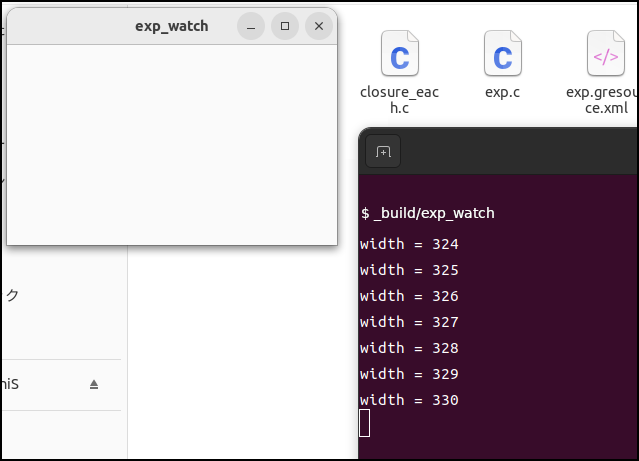
\includegraphics[width=9.6cm,height=6.9cm]{../image/exp_watch.png}
\caption{exp\_watch}
\end{figure}

When you resize the window, the width is displayed in the terminal.

\begin{lstlisting}[language=C, numbers=left]
#include <gtk/gtk.h>

GtkExpression *expression;
GtkExpressionWatch *watch;

static void
notify (gpointer user_data) {
  GValue value = G_VALUE_INIT;

  if (gtk_expression_watch_evaluate (watch, &value))
    g_print ("width = %d\n", g_value_get_int (&value));
  else
    g_print ("evaluation failed.\n");
}

static int
close_request_cb (GtkWindow *win) {
  gtk_expression_watch_unwatch (watch);
  gtk_expression_unref (expression);
  return false;
}

static void
app_activate (GApplication *application) {
  GtkApplication *app = GTK_APPLICATION (application);
  gtk_window_present (gtk_application_get_active_window(app));
}

static void
app_startup (GApplication *application) {
  GtkApplication *app = GTK_APPLICATION (application);
  GtkWidget *win;

  win = GTK_WIDGET (gtk_application_window_new (app));
  g_signal_connect (win, "close-request", G_CALLBACK (close_request_cb), NULL);

  expression = gtk_property_expression_new (GTK_TYPE_WINDOW, NULL, "default-width");
  watch = gtk_expression_watch (expression, win, notify, NULL, NULL);
}

#define APPLICATION_ID "com.github.ToshioCP.exp_watch"

int
main (int argc, char **argv) {
  GtkApplication *app;
  int stat;

  app = gtk_application_new (APPLICATION_ID, G_APPLICATION_DEFAULT_FLAGS);

  g_signal_connect (app, "startup", G_CALLBACK (app_startup), NULL);
  g_signal_connect (app, "activate", G_CALLBACK (app_activate), NULL);

  stat =g_application_run (G_APPLICATION (app), argc, argv);
  g_object_unref (app);
  return stat;
}
\end{lstlisting}

\begin{itemize}
\tightlist
\item
  37: A property expression looks up the ``default-width'' property of
  the window.
\item
  38: Create a watch structure for the expression. The callback
  \passthrough{\lstinline!notify!} is called every time the value of the
  expression changes. The `this' object is
  \passthrough{\lstinline!win!}, so the expression returns the default
  width of the window.
\item
  6-14: The callback function \passthrough{\lstinline!notify!}. It uses
  \passthrough{\lstinline!gtk\_expression\_watch\_evaluate!} to get the
  value of the expression. The `this' object is given in advance (when
  the watch is created). It outputs the window width to the standard
  output.
\item
  16-21: A handler for the ``close-request''signal on the window. It
  stops the watch. In addition, it releases the reference to the
  expression. Because \passthrough{\lstinline!gtk\_expression\_watch!}
  doesn't take the ownership of the expression, you own it. So, the
  release is necessary.
\end{itemize}

\subsection{Gtkexpression in ui files}\label{gtkexpression-in-ui-files}

GtkBuilder supports GtkExpressions. There are four tags.

\begin{itemize}
\tightlist
\item
  constant tag to create constant expression. Type attribute specifies
  the type name of the value. If no type is specified, the type is
  assumed to be an object. The content is the value of the expression.
\item
  lookup tag to create property expression. Type attribute specifies the
  type of the object. Name attribute specifies the property name. The
  content is an expression or object which has the property to look up.
  If there's no content, `this' object is used.
\item
  closure tag to create closure expression. Type attribute specifies the
  type of the returned value. Function attribute specifies the callback
  function. The contents of the tag are arguments that are expressions.
\item
  binding tag to bind a property to an expression. It is put in the
  content of an object tag. Name attribute specifies the property name
  of the object. The content is an expression.
\end{itemize}

\begin{lstlisting}[language=XML]
<constant type="gchararray">Hello world</constant>
<lookup name="label" type="GtkLabel">label</lookup>
<closure type="gint" function="callback_function"></closure>
<bind name="label">
  <lookup name="default-width">win</lookup>
</bind>
\end{lstlisting}

These tags are usually used for GtkBuilderListItemFactory.

\begin{lstlisting}[language=XML]
<interface>
  <template class="GtkListItem">
    <property name="child">
      <object class="GtkLabel">
        <binding name="label">
          <lookup name="string" type="GtkStringObject">
            <lookup name="item">GtkListItem</lookup>
          </lookup>
        </binding>
      </object>
    </property>
  </template>
</interface>
\end{lstlisting}

GtkBuilderListItemFactory uses GtkBuilder to extends the GtkListItem
with the XML data.

In the xml file above, ``GtkListItem'' is an instance of the GtkListItem
template. It is the `this' object given to the expressions. (The
information is in the \href{https://blog.gtk.org/2020/09/}{GTK
Development Blog}).

GtkBuilder calls \passthrough{\lstinline!gtk\_expression\_bind!}
function when it finds a binding tag. The function sets the `this'
object like this:

\begin{enumerate}
\def\labelenumi{\arabic{enumi}.}
\tightlist
\item
  If the binding tag has object attribute, the object will be the `this'
  object.
\item
  If the current object of the GtkBuilder exists, it will be the `this'
  object. That's why a GtkListItem instance is the `this' object of the
  XML data for a GtkBuilderListItemFactory.
\item
  Otherwise, the target object of the binding tag will be the `this'
  object.
\end{enumerate}

GTK 4 document doesn't describe information about ``this'' object when
expressions are defined in a ui file. The information above is found
from the GTK 4 source files and it is possible to include mistakes. If
you have accurate information, please let me know.

A sample program \passthrough{\lstinline!exp.c!} and a ui file
\passthrough{\lstinline!exp.ui!} is in
\passthrough{\lstinline!src/expression!} directory. The ui file includes
lookup, closure and bind tags. No constant tag is included. However,
constant tags are not used so often.

\begin{figure}
\centering
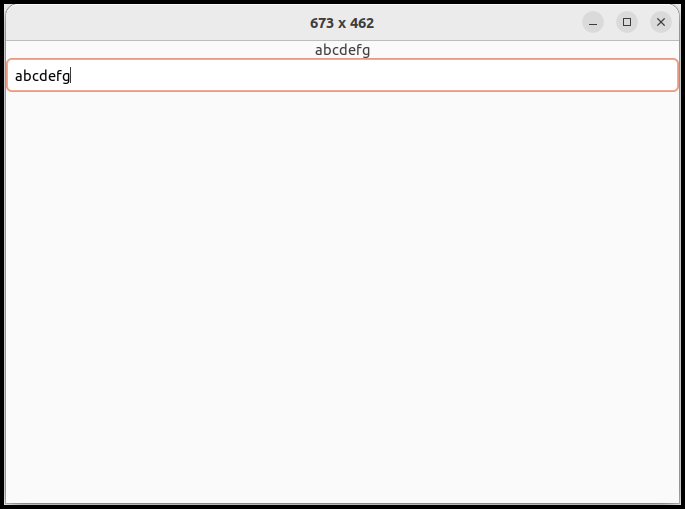
\includegraphics[width=10.3cm,height=7.6cm]{../image/exp.png}
\caption{exp.c}
\end{figure}

If you resize the window, the size is shown at the title of the window.
If you type characters in the entry, the same characters appear on the
label.

The ui file is as follows.

\begin{lstlisting}[language=XML, numbers=left]
<?xml version="1.0" encoding="UTF-8"?>
<interface>
  <object class="GtkApplicationWindow" id="win">
    <binding name="title">
      <closure type="gchararray" function="set_title">
        <lookup name="default-width" type="GtkWindow"></lookup>
        <lookup name="default-height" type="GtkWindow"></lookup>
      </closure>
    </binding>
    <property name="default-width">600</property>
    <property name="default-height">400</property>
    <child>
      <object class="GtkBox">
        <property name="orientation">GTK_ORIENTATION_VERTICAL</property>
        <child>
          <object class="GtkLabel">
            <binding name="label">
              <lookup name="text">
                buffer
              </lookup>
            </binding>
          </object>
        </child>
        <child>
          <object class="GtkEntry">
            <property name="buffer">
              <object class="GtkEntryBuffer" id="buffer"></object>
            </property>
          </object>
        </child>
      </object>
    </child>
  </object>
</interface>
\end{lstlisting}

\begin{itemize}
\tightlist
\item
  4-9: The title property of the main window is bound to a closure
  expression. Its callback function \passthrough{\lstinline!set\_title!}
  is defined in the C source file. It returns a string because the type
  attribute of the tag is ``gchararray''. Two parameters are given to
  the function. They are width and height of the window. Lookup tags
  don't have contents, so `this' object is used to look up the
  properties. The `this' object is \passthrough{\lstinline!win!}, which
  is the target of the binding (\passthrough{\lstinline!win!} includes
  the binding tag).
\item
  17-21: The ``label'' property of the GtkLabel instance is bound to the
  ``text'' property of \passthrough{\lstinline!buffer!}, which is the
  buffer of GtkEntry defined in line 25. If a user types characters in
  the entry, the same characters appear on the label.
\end{itemize}

The C source file is as follows.

\begin{lstlisting}[language=C, numbers=left]
#include <gtk/gtk.h>

char *
set_title (GtkWidget *win, int width, int height) {
  return g_strdup_printf ("%d x %d", width, height);
}

static void
app_activate (GApplication *application) {
  GtkApplication *app = GTK_APPLICATION (application);
  gtk_window_present (gtk_application_get_active_window(app));
}

static void
app_startup (GApplication *application) {
  GtkApplication *app = GTK_APPLICATION (application);
  GtkBuilder *build;
  GtkWidget *win;

  build = gtk_builder_new_from_resource ("/com/github/ToshioCP/exp/exp.ui");
  win = GTK_WIDGET (gtk_builder_get_object (build, "win"));
  gtk_window_set_application (GTK_WINDOW (win), app);
  g_object_unref (build);
}

#define APPLICATION_ID "com.github.ToshioCP.exp"

int
main (int argc, char **argv) {
  GtkApplication *app;
  int stat;

  app = gtk_application_new (APPLICATION_ID, G_APPLICATION_DEFAULT_FLAGS);

  g_signal_connect (app, "startup", G_CALLBACK (app_startup), NULL);
  g_signal_connect (app, "activate", G_CALLBACK (app_activate), NULL);

  stat =g_application_run (G_APPLICATION (app), argc, argv);
  g_object_unref (app);
  return stat;
}
\end{lstlisting}

\begin{itemize}
\tightlist
\item
  4-6: The callback function. It returns a string (w)x(h), where the w
  and h are the width and height of the window. String duplication is
  necessary.
\end{itemize}

The C source file is very simple because almost everything is done in
the ui file.

\subsection{Conversion between
GValues}\label{conversion-between-gvalues}

If you bind different type properties, type conversion is automatically
done. Suppose a label property (string) is bound to default-width
property (int).

\begin{lstlisting}[language=XML]
<object class="GtkLabel">
  <binding name="label">
    <lookup name="default-width">
      win
    </lookup>
  </binding>
</object>
\end{lstlisting}

The expression created by the lookup tag returns a int type GValue. On
the other hand ``label'' property holds a string type GValue. When a
GValue is copied to another GValue, the type is automatically converted
if possible. If the current width is 100, an int
\passthrough{\lstinline!100!} is converted to a string
\passthrough{\lstinline!"100"!}.

If you use \passthrough{\lstinline!g\_object\_get!} and
\passthrough{\lstinline!g\_object\_set!} to copy properties, the value
is automatically converted.

\subsection{Meson.build}\label{meson.build}

The source files are in \passthrough{\lstinline!src/expression!}
directory. You can build all the files at once.

\begin{lstlisting}
$ cd src/expression
$ meson setup _build
$ ninja -C _build
\end{lstlisting}

For example, if you want to run ``exp'', which is the executable file
from ``exp.c'', type \passthrough{\lstinline!\_build/exp!}. You can run
other programs as well.

The file \passthrough{\lstinline!meson.build!} is as follows.

\begin{lstlisting}[numbers=left]
project('exp', 'c')

gtkdep = dependency('gtk4')

gnome=import('gnome')
resources = gnome.compile_resources('resources','exp.gresource.xml')

sourcefiles=files('exp.c')

executable('exp', sourcefiles, resources, dependencies: gtkdep, export_dynamic: true, install: false)
executable('exp_constant', 'exp_constant.c', dependencies: gtkdep, export_dynamic: true, install: false)
executable('exp_constant_simple', 'exp_constant_simple.c', dependencies: gtkdep, export_dynamic: true, install: false)
executable('exp_property_simple', 'exp_property_simple.c', dependencies: gtkdep, export_dynamic: true, install: false)
executable('closure', 'closure.c', dependencies: gtkdep, export_dynamic: true, install: false)
executable('closure_each', 'closure_each.c', dependencies: gtkdep, export_dynamic: true, install: false)
executable('exp_closure_simple', 'exp_closure_simple.c', dependencies: gtkdep, export_dynamic: true, install: false)
executable('exp_closure_with_error_report', 'exp_closure_with_error_report.c', dependencies: gtkdep, export_dynamic: true, install: false)
executable('exp_bind', 'exp_bind.c', resources, dependencies: gtkdep, export_dynamic: true, install: false)
executable('exp_watch', 'exp_watch.c', dependencies: gtkdep, export_dynamic: true, install: false)
executable('exp_test', 'exp_test.c', resources, dependencies: gtkdep, export_dynamic: true, install: false)
\end{lstlisting}
